% Options for packages loaded elsewhere
\PassOptionsToPackage{unicode}{hyperref}
\PassOptionsToPackage{hyphens}{url}
\PassOptionsToPackage{dvipsnames,svgnames,x11names}{xcolor}
%
\documentclass[
  letterpaper,
  DIV=11,
  numbers=noendperiod]{scrartcl}

\usepackage{amsmath,amssymb}
\usepackage{iftex}
\ifPDFTeX
  \usepackage[T1]{fontenc}
  \usepackage[utf8]{inputenc}
  \usepackage{textcomp} % provide euro and other symbols
\else % if luatex or xetex
  \usepackage{unicode-math}
  \defaultfontfeatures{Scale=MatchLowercase}
  \defaultfontfeatures[\rmfamily]{Ligatures=TeX,Scale=1}
\fi
\usepackage{lmodern}
\ifPDFTeX\else  
    % xetex/luatex font selection
\fi
% Use upquote if available, for straight quotes in verbatim environments
\IfFileExists{upquote.sty}{\usepackage{upquote}}{}
\IfFileExists{microtype.sty}{% use microtype if available
  \usepackage[]{microtype}
  \UseMicrotypeSet[protrusion]{basicmath} % disable protrusion for tt fonts
}{}
\makeatletter
\@ifundefined{KOMAClassName}{% if non-KOMA class
  \IfFileExists{parskip.sty}{%
    \usepackage{parskip}
  }{% else
    \setlength{\parindent}{0pt}
    \setlength{\parskip}{6pt plus 2pt minus 1pt}}
}{% if KOMA class
  \KOMAoptions{parskip=half}}
\makeatother
\usepackage{xcolor}
\setlength{\emergencystretch}{3em} % prevent overfull lines
\setcounter{secnumdepth}{5}
% Make \paragraph and \subparagraph free-standing
\makeatletter
\ifx\paragraph\undefined\else
  \let\oldparagraph\paragraph
  \renewcommand{\paragraph}{
    \@ifstar
      \xxxParagraphStar
      \xxxParagraphNoStar
  }
  \newcommand{\xxxParagraphStar}[1]{\oldparagraph*{#1}\mbox{}}
  \newcommand{\xxxParagraphNoStar}[1]{\oldparagraph{#1}\mbox{}}
\fi
\ifx\subparagraph\undefined\else
  \let\oldsubparagraph\subparagraph
  \renewcommand{\subparagraph}{
    \@ifstar
      \xxxSubParagraphStar
      \xxxSubParagraphNoStar
  }
  \newcommand{\xxxSubParagraphStar}[1]{\oldsubparagraph*{#1}\mbox{}}
  \newcommand{\xxxSubParagraphNoStar}[1]{\oldsubparagraph{#1}\mbox{}}
\fi
\makeatother

\usepackage{color}
\usepackage{fancyvrb}
\newcommand{\VerbBar}{|}
\newcommand{\VERB}{\Verb[commandchars=\\\{\}]}
\DefineVerbatimEnvironment{Highlighting}{Verbatim}{commandchars=\\\{\}}
% Add ',fontsize=\small' for more characters per line
\usepackage{framed}
\definecolor{shadecolor}{RGB}{241,243,245}
\newenvironment{Shaded}{\begin{snugshade}}{\end{snugshade}}
\newcommand{\AlertTok}[1]{\textcolor[rgb]{0.68,0.00,0.00}{#1}}
\newcommand{\AnnotationTok}[1]{\textcolor[rgb]{0.37,0.37,0.37}{#1}}
\newcommand{\AttributeTok}[1]{\textcolor[rgb]{0.40,0.45,0.13}{#1}}
\newcommand{\BaseNTok}[1]{\textcolor[rgb]{0.68,0.00,0.00}{#1}}
\newcommand{\BuiltInTok}[1]{\textcolor[rgb]{0.00,0.23,0.31}{#1}}
\newcommand{\CharTok}[1]{\textcolor[rgb]{0.13,0.47,0.30}{#1}}
\newcommand{\CommentTok}[1]{\textcolor[rgb]{0.37,0.37,0.37}{#1}}
\newcommand{\CommentVarTok}[1]{\textcolor[rgb]{0.37,0.37,0.37}{\textit{#1}}}
\newcommand{\ConstantTok}[1]{\textcolor[rgb]{0.56,0.35,0.01}{#1}}
\newcommand{\ControlFlowTok}[1]{\textcolor[rgb]{0.00,0.23,0.31}{\textbf{#1}}}
\newcommand{\DataTypeTok}[1]{\textcolor[rgb]{0.68,0.00,0.00}{#1}}
\newcommand{\DecValTok}[1]{\textcolor[rgb]{0.68,0.00,0.00}{#1}}
\newcommand{\DocumentationTok}[1]{\textcolor[rgb]{0.37,0.37,0.37}{\textit{#1}}}
\newcommand{\ErrorTok}[1]{\textcolor[rgb]{0.68,0.00,0.00}{#1}}
\newcommand{\ExtensionTok}[1]{\textcolor[rgb]{0.00,0.23,0.31}{#1}}
\newcommand{\FloatTok}[1]{\textcolor[rgb]{0.68,0.00,0.00}{#1}}
\newcommand{\FunctionTok}[1]{\textcolor[rgb]{0.28,0.35,0.67}{#1}}
\newcommand{\ImportTok}[1]{\textcolor[rgb]{0.00,0.46,0.62}{#1}}
\newcommand{\InformationTok}[1]{\textcolor[rgb]{0.37,0.37,0.37}{#1}}
\newcommand{\KeywordTok}[1]{\textcolor[rgb]{0.00,0.23,0.31}{\textbf{#1}}}
\newcommand{\NormalTok}[1]{\textcolor[rgb]{0.00,0.23,0.31}{#1}}
\newcommand{\OperatorTok}[1]{\textcolor[rgb]{0.37,0.37,0.37}{#1}}
\newcommand{\OtherTok}[1]{\textcolor[rgb]{0.00,0.23,0.31}{#1}}
\newcommand{\PreprocessorTok}[1]{\textcolor[rgb]{0.68,0.00,0.00}{#1}}
\newcommand{\RegionMarkerTok}[1]{\textcolor[rgb]{0.00,0.23,0.31}{#1}}
\newcommand{\SpecialCharTok}[1]{\textcolor[rgb]{0.37,0.37,0.37}{#1}}
\newcommand{\SpecialStringTok}[1]{\textcolor[rgb]{0.13,0.47,0.30}{#1}}
\newcommand{\StringTok}[1]{\textcolor[rgb]{0.13,0.47,0.30}{#1}}
\newcommand{\VariableTok}[1]{\textcolor[rgb]{0.07,0.07,0.07}{#1}}
\newcommand{\VerbatimStringTok}[1]{\textcolor[rgb]{0.13,0.47,0.30}{#1}}
\newcommand{\WarningTok}[1]{\textcolor[rgb]{0.37,0.37,0.37}{\textit{#1}}}

\providecommand{\tightlist}{%
  \setlength{\itemsep}{0pt}\setlength{\parskip}{0pt}}\usepackage{longtable,booktabs,array}
\usepackage{calc} % for calculating minipage widths
% Correct order of tables after \paragraph or \subparagraph
\usepackage{etoolbox}
\makeatletter
\patchcmd\longtable{\par}{\if@noskipsec\mbox{}\fi\par}{}{}
\makeatother
% Allow footnotes in longtable head/foot
\IfFileExists{footnotehyper.sty}{\usepackage{footnotehyper}}{\usepackage{footnote}}
\makesavenoteenv{longtable}
\usepackage{graphicx}
\makeatletter
\def\maxwidth{\ifdim\Gin@nat@width>\linewidth\linewidth\else\Gin@nat@width\fi}
\def\maxheight{\ifdim\Gin@nat@height>\textheight\textheight\else\Gin@nat@height\fi}
\makeatother
% Scale images if necessary, so that they will not overflow the page
% margins by default, and it is still possible to overwrite the defaults
% using explicit options in \includegraphics[width, height, ...]{}
\setkeys{Gin}{width=\maxwidth,height=\maxheight,keepaspectratio}
% Set default figure placement to htbp
\makeatletter
\def\fps@figure{htbp}
\makeatother

\KOMAoption{captions}{tableheading}
\makeatletter
\@ifpackageloaded{caption}{}{\usepackage{caption}}
\AtBeginDocument{%
\ifdefined\contentsname
  \renewcommand*\contentsname{Table of contents}
\else
  \newcommand\contentsname{Table of contents}
\fi
\ifdefined\listfigurename
  \renewcommand*\listfigurename{List of Figures}
\else
  \newcommand\listfigurename{List of Figures}
\fi
\ifdefined\listtablename
  \renewcommand*\listtablename{List of Tables}
\else
  \newcommand\listtablename{List of Tables}
\fi
\ifdefined\figurename
  \renewcommand*\figurename{Figure}
\else
  \newcommand\figurename{Figure}
\fi
\ifdefined\tablename
  \renewcommand*\tablename{Table}
\else
  \newcommand\tablename{Table}
\fi
}
\@ifpackageloaded{float}{}{\usepackage{float}}
\floatstyle{ruled}
\@ifundefined{c@chapter}{\newfloat{codelisting}{h}{lop}}{\newfloat{codelisting}{h}{lop}[chapter]}
\floatname{codelisting}{Listing}
\newcommand*\listoflistings{\listof{codelisting}{List of Listings}}
\makeatother
\makeatletter
\makeatother
\makeatletter
\@ifpackageloaded{caption}{}{\usepackage{caption}}
\@ifpackageloaded{subcaption}{}{\usepackage{subcaption}}
\makeatother

\ifLuaTeX
  \usepackage{selnolig}  % disable illegal ligatures
\fi
\usepackage{bookmark}

\IfFileExists{xurl.sty}{\usepackage{xurl}}{} % add URL line breaks if available
\urlstyle{same} % disable monospaced font for URLs
\hypersetup{
  pdftitle={Trends in Death License: Analyzing the Distribution of Death Licenses in Great Toronto Area in the Past Decade and Potentional Realation to the Extreme Weather and Covid-19},
  pdfauthor={Shanjie Jiao; Carrie Su},
  colorlinks=true,
  linkcolor={blue},
  filecolor={Maroon},
  citecolor={Blue},
  urlcolor={Blue},
  pdfcreator={LaTeX via pandoc}}


\title{Trends in Death License: Analyzing the Distribution of Death
Licenses in Great Toronto Area in the Past Decade and Potentional
Realation to the Extreme Weather and Covid-19\thanks{Code and data are
available at: https://github.com/Jie-jiao05/Paper-1.git}}
\author{Shanjie Jiao \and Carrie Su}
\date{October 14, 2025}

\begin{document}
\maketitle
\begin{abstract}
Urbanization amplified the inequality between urban area and rural area,
in various aspects, including population density, economic growth,
infrastructure, and public health services. During 2019-2023 the
global-wide public health panic Covid-19 and the rising number in
extreme weather, all it cause the rising mortality not just in Toronto,
also global wide. As death number and death license are two relatively
separate concept. It is obvious that the Covid-19 and severe climate
have positive correlation with number of death record, while number of
death license only show a positive relation with severe weather in
January specifically and uncorrelated with Covid-19, by analyzing
Toronto and Outside City Limits data.
\end{abstract}


\begin{verbatim}
Rows: 252 Columns: 2
-- Column specification --------------------------------------------------------
Delimiter: ","
chr (1): Country
dbl (1): FertilityRate_2023

i Use `spec()` to retrieve the full column specification for this data.
i Specify the column types or set `show_col_types = FALSE` to quiet this message.
\end{verbatim}

\begin{verbatim}
Warning: st_centroid assumes attributes are constant over geometries
\end{verbatim}

\begin{verbatim}
Warning: The `size` argument of `element_line()` is deprecated as of ggplot2 3.4.0.
i Please use the `linewidth` argument instead.
\end{verbatim}

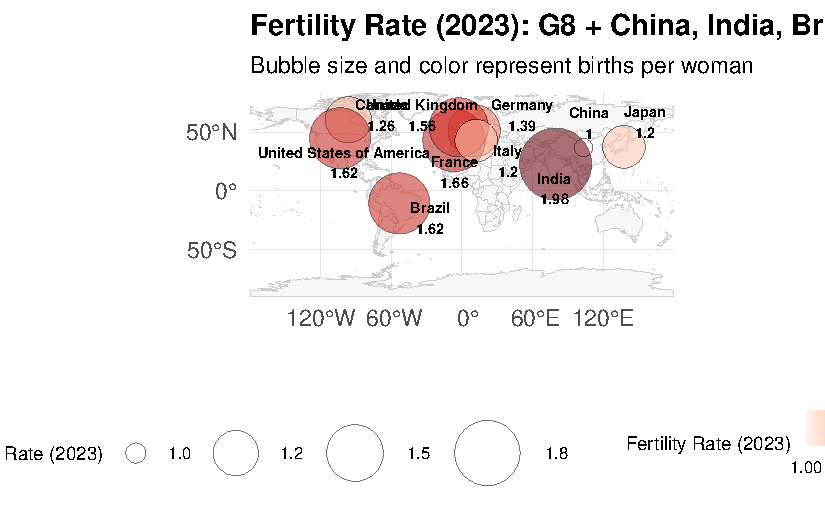
\includegraphics{paper_files/figure-pdf/unnamed-chunk-2-1.pdf}

\begin{Shaded}
\begin{Highlighting}[]
\FunctionTok{library}\NormalTok{(stringr)}
\end{Highlighting}
\end{Shaded}

\begin{verbatim}
Warning: package 'stringr' was built under R version 4.4.3
\end{verbatim}

\begin{Shaded}
\begin{Highlighting}[]
\FunctionTok{library}\NormalTok{(scico)}
\end{Highlighting}
\end{Shaded}

\begin{verbatim}
Warning: package 'scico' was built under R version 4.4.3
\end{verbatim}

\begin{Shaded}
\begin{Highlighting}[]
\NormalTok{fert\_per\_prov }\OtherTok{\textless{}{-}} \FunctionTok{read\_csv}\NormalTok{(}\FunctionTok{here}\NormalTok{(}\StringTok{"fert\_per\_province.csv"}\NormalTok{))}
\end{Highlighting}
\end{Shaded}

\begin{verbatim}
Rows: 4347 Columns: 15
-- Column specification --------------------------------------------------------
Delimiter: ","
chr (7): GEO, DGUID, Characteristics, UOM, SCALAR_FACTOR, VECTOR, STATUS
dbl (6): REF_DATE, UOM_ID, SCALAR_ID, COORDINATE, VALUE, DECIMALS
lgl (2): SYMBOL, TERMINATED

i Use `spec()` to retrieve the full column specification for this data.
i Specify the column types or set `show_col_types = FALSE` to quiet this message.
\end{verbatim}

\begin{Shaded}
\begin{Highlighting}[]
\NormalTok{fert\_2023 }\OtherTok{\textless{}{-}}\NormalTok{ fert\_per\_prov }\SpecialCharTok{\%\textgreater{}\%}
  \FunctionTok{filter}\NormalTok{(}
\NormalTok{    REF\_DATE }\SpecialCharTok{==} \DecValTok{2023}\NormalTok{,}
    \FunctionTok{grepl}\NormalTok{(}\StringTok{"total fertility rate"}\NormalTok{, Characteristics, }\AttributeTok{ignore.case =} \ConstantTok{TRUE}\NormalTok{)}
\NormalTok{  )}

\CommentTok{\# ==== Step 3: Select relevant columns (Province, Year, and Value) ====}
\NormalTok{fert\_2023\_summary }\OtherTok{\textless{}{-}}\NormalTok{ fert\_2023 }\SpecialCharTok{\%\textgreater{}\%}
  \FunctionTok{select}\NormalTok{(GEO, REF\_DATE, Characteristics, VALUE)}



\CommentTok{\# ==== Step 3: Clean province names ====}
\NormalTok{fert\_2023\_summary }\OtherTok{\textless{}{-}}\NormalTok{ fert\_2023\_summary }\SpecialCharTok{\%\textgreater{}\%}
  \FunctionTok{mutate}\NormalTok{(}
    \AttributeTok{GEO\_clean =}\NormalTok{ GEO }\SpecialCharTok{\%\textgreater{}\%}
      \FunctionTok{str\_replace}\NormalTok{(}\StringTok{", place of residence of mother"}\NormalTok{, }\StringTok{""}\NormalTok{) }\SpecialCharTok{\%\textgreater{}\%}
      \FunctionTok{str\_trim}\NormalTok{()}
\NormalTok{  )}

\CommentTok{\# ==== Step 4: Load the map ====}
\NormalTok{canada }\OtherTok{\textless{}{-}} \FunctionTok{ne\_states}\NormalTok{(}\AttributeTok{country =} \StringTok{"canada"}\NormalTok{, }\AttributeTok{returnclass =} \StringTok{"sf"}\NormalTok{)}

\CommentTok{\# ==== Step 5: Manual name reconciliation ====}
\CommentTok{\# Ensure names match exactly between GEO\_clean and canada$name}
\NormalTok{name\_map }\OtherTok{\textless{}{-}} \FunctionTok{c}\NormalTok{(}
  \StringTok{"Newfoundland and Labrador"} \OtherTok{=} \StringTok{"Newfoundland and Labrador"}\NormalTok{,}
  \StringTok{"Prince Edward Island"} \OtherTok{=} \StringTok{"Prince Edward Island"}\NormalTok{,}
  \StringTok{"Nova Scotia"} \OtherTok{=} \StringTok{"Nova Scotia"}\NormalTok{,}
  \StringTok{"New Brunswick"} \OtherTok{=} \StringTok{"New Brunswick"}\NormalTok{,}
  \StringTok{"Quebec"} \OtherTok{=} \StringTok{"Québec"}\NormalTok{,}
  \StringTok{"Ontario"} \OtherTok{=} \StringTok{"Ontario"}\NormalTok{,}
  \StringTok{"Manitoba"} \OtherTok{=} \StringTok{"Manitoba"}\NormalTok{,}
  \StringTok{"Saskatchewan"} \OtherTok{=} \StringTok{"Saskatchewan"}\NormalTok{,}
  \StringTok{"Alberta"} \OtherTok{=} \StringTok{"Alberta"}\NormalTok{,}
  \StringTok{"British Columbia"} \OtherTok{=} \StringTok{"British Columbia"}\NormalTok{,}
  \StringTok{"Yukon"} \OtherTok{=} \StringTok{"Yukon"}\NormalTok{,}
  \StringTok{"Northwest Territories"} \OtherTok{=} \StringTok{"Northwest Territories"}\NormalTok{,}
  \StringTok{"Nunavut"} \OtherTok{=} \StringTok{"Nunavut"}
\NormalTok{)}

\NormalTok{fert\_2023\_summary }\OtherTok{\textless{}{-}}\NormalTok{ fert\_2023\_summary }\SpecialCharTok{\%\textgreater{}\%}
  \FunctionTok{mutate}\NormalTok{(}\AttributeTok{GEO\_match =} \FunctionTok{recode}\NormalTok{(GEO\_clean, }\SpecialCharTok{!!!}\NormalTok{name\_map))}

\CommentTok{\# ==== Step 6: Join with map ====}
\NormalTok{canada\_map }\OtherTok{\textless{}{-}}\NormalTok{ canada }\SpecialCharTok{\%\textgreater{}\%}
  \FunctionTok{left\_join}\NormalTok{(fert\_2023\_summary, }\AttributeTok{by =} \FunctionTok{c}\NormalTok{(}\StringTok{"name"} \OtherTok{=} \StringTok{"GEO\_match"}\NormalTok{))}

\CommentTok{\# ==== Step 7: Verify missing provinces ====}
\FunctionTok{print}\NormalTok{(}\FunctionTok{setdiff}\NormalTok{(canada}\SpecialCharTok{$}\NormalTok{name, canada\_map}\SpecialCharTok{$}\NormalTok{name[}\SpecialCharTok{!}\FunctionTok{is.na}\NormalTok{(canada\_map}\SpecialCharTok{$}\NormalTok{VALUE)]))}
\end{Highlighting}
\end{Shaded}

\begin{verbatim}
character(0)
\end{verbatim}

\begin{Shaded}
\begin{Highlighting}[]
\FunctionTok{ggplot}\NormalTok{(canada\_map) }\SpecialCharTok{+}
  \FunctionTok{geom\_sf}\NormalTok{(}\FunctionTok{aes}\NormalTok{(}\AttributeTok{fill =}\NormalTok{ VALUE), }\AttributeTok{color =} \StringTok{"white"}\NormalTok{, }\AttributeTok{linewidth =} \FloatTok{0.3}\NormalTok{) }\SpecialCharTok{+}
  \FunctionTok{geom\_sf\_text}\NormalTok{(}
    \FunctionTok{aes}\NormalTok{(}\AttributeTok{label =} \FunctionTok{round}\NormalTok{(VALUE, }\DecValTok{2}\NormalTok{)),}
    \AttributeTok{color =} \StringTok{"black"}\NormalTok{,}
    \AttributeTok{size =} \FloatTok{3.5}\NormalTok{,}
    \AttributeTok{check\_overlap =} \ConstantTok{TRUE}
\NormalTok{  ) }\SpecialCharTok{+}
  \FunctionTok{scale\_fill\_gradient}\NormalTok{(}
    \AttributeTok{low =} \StringTok{"\#FDE0DD"}\NormalTok{,   }\CommentTok{\# light red}
    \AttributeTok{high =} \StringTok{"\#99000D"}\NormalTok{,  }\CommentTok{\# dark red}
    \AttributeTok{name =} \StringTok{"Fertility Rate}\SpecialCharTok{\textbackslash{}n}\StringTok{(children per woman)"}\NormalTok{,}
    \AttributeTok{na.value =} \StringTok{"grey90"}
\NormalTok{  ) }\SpecialCharTok{+}
  \FunctionTok{labs}\NormalTok{(}
    \AttributeTok{title =} \StringTok{"Total Fertility Rate by Province (2023)"}\NormalTok{,}
    \AttributeTok{caption =} \StringTok{"Source: Statistics Canada"}
\NormalTok{  ) }\SpecialCharTok{+}
  \FunctionTok{theme\_minimal}\NormalTok{(}\AttributeTok{base\_size =} \DecValTok{13}\NormalTok{) }\SpecialCharTok{+}
  \FunctionTok{theme}\NormalTok{(}
    \AttributeTok{legend.position =} \StringTok{"right"}\NormalTok{,}
    \AttributeTok{axis.text =} \FunctionTok{element\_blank}\NormalTok{(),       }\CommentTok{\# remove axis text}
    \AttributeTok{axis.ticks =} \FunctionTok{element\_blank}\NormalTok{(),      }\CommentTok{\# remove axis ticks}
    \AttributeTok{axis.title =} \FunctionTok{element\_blank}\NormalTok{(),      }\CommentTok{\# remove x and y labels}
    \AttributeTok{panel.grid =} \FunctionTok{element\_blank}\NormalTok{(),      }\CommentTok{\# remove grid lines}
    \AttributeTok{plot.title =} \FunctionTok{element\_text}\NormalTok{(}\AttributeTok{face =} \StringTok{"bold"}\NormalTok{, }\AttributeTok{size =} \DecValTok{16}\NormalTok{),}
    \AttributeTok{plot.subtitle =} \FunctionTok{element\_text}\NormalTok{(}\AttributeTok{size =} \DecValTok{12}\NormalTok{)}
\NormalTok{  )}
\end{Highlighting}
\end{Shaded}

\begin{verbatim}
Warning in st_point_on_surface.sfc(sf::st_zm(x)): st_point_on_surface may not
give correct results for longitude/latitude data
\end{verbatim}

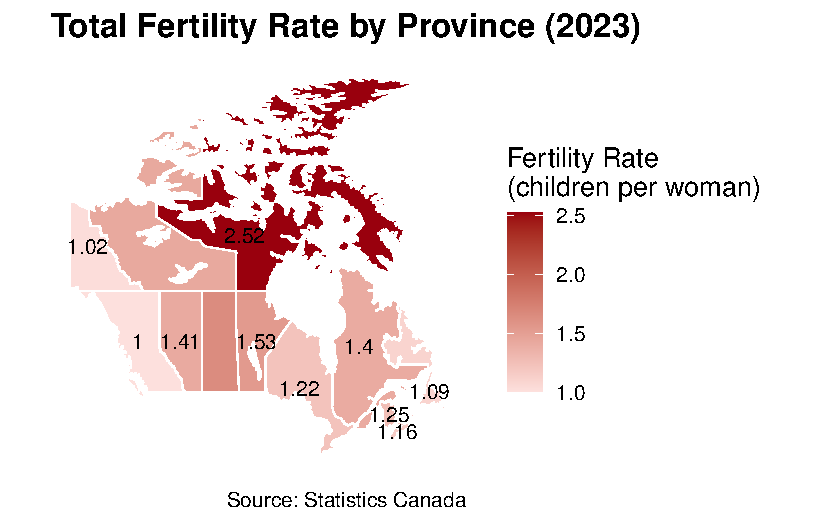
\includegraphics{paper_files/figure-pdf/unnamed-chunk-3-1.pdf}

\begin{Shaded}
\begin{Highlighting}[]
\FunctionTok{library}\NormalTok{(readxl)}
\end{Highlighting}
\end{Shaded}

\begin{verbatim}
Warning: package 'readxl' was built under R version 4.4.3
\end{verbatim}

\begin{Shaded}
\begin{Highlighting}[]
\NormalTok{fertility\_trend }\OtherTok{\textless{}{-}} \FunctionTok{read\_excel}\NormalTok{(}\FunctionTok{here}\NormalTok{(}\StringTok{"Canada\_Fertility\_1921\_2022.xlsx"}\NormalTok{))}

\NormalTok{fertility\_postWWII }\OtherTok{\textless{}{-}}\NormalTok{ fertility\_trend }\SpecialCharTok{\%\textgreater{}\%}
  \FunctionTok{filter}\NormalTok{(Year }\SpecialCharTok{\textgreater{}=} \DecValTok{1946}\NormalTok{)}

\FunctionTok{ggplot}\NormalTok{(fertility\_postWWII, }\FunctionTok{aes}\NormalTok{(}\AttributeTok{x =}\NormalTok{ Year)) }\SpecialCharTok{+}
  \CommentTok{\# Highlight selected historical/economic events after 1946}
  \FunctionTok{annotate}\NormalTok{(}\StringTok{"rect"}\NormalTok{, }\AttributeTok{xmin =} \DecValTok{1947}\NormalTok{, }\AttributeTok{xmax =} \DecValTok{1948}\NormalTok{, }\AttributeTok{ymin =} \SpecialCharTok{{-}}\ConstantTok{Inf}\NormalTok{, }\AttributeTok{ymax =} \ConstantTok{Inf}\NormalTok{,}
           \AttributeTok{fill =} \StringTok{"grey70"}\NormalTok{, }\AttributeTok{alpha =} \FloatTok{0.2}\NormalTok{) }\SpecialCharTok{+}
  \FunctionTok{annotate}\NormalTok{(}\StringTok{"rect"}\NormalTok{, }\AttributeTok{xmin =} \DecValTok{1953}\NormalTok{, }\AttributeTok{xmax =} \DecValTok{1954}\NormalTok{, }\AttributeTok{ymin =} \SpecialCharTok{{-}}\ConstantTok{Inf}\NormalTok{, }\AttributeTok{ymax =} \ConstantTok{Inf}\NormalTok{,}
           \AttributeTok{fill =} \StringTok{"grey70"}\NormalTok{, }\AttributeTok{alpha =} \FloatTok{0.2}\NormalTok{) }\SpecialCharTok{+}
  \FunctionTok{annotate}\NormalTok{(}\StringTok{"rect"}\NormalTok{, }\AttributeTok{xmin =} \DecValTok{1974}\NormalTok{, }\AttributeTok{xmax =} \DecValTok{1975}\NormalTok{, }\AttributeTok{ymin =} \SpecialCharTok{{-}}\ConstantTok{Inf}\NormalTok{, }\AttributeTok{ymax =} \ConstantTok{Inf}\NormalTok{,}
           \AttributeTok{fill =} \StringTok{"grey70"}\NormalTok{, }\AttributeTok{alpha =} \FloatTok{0.2}\NormalTok{) }\SpecialCharTok{+}
  \FunctionTok{annotate}\NormalTok{(}\StringTok{"rect"}\NormalTok{, }\AttributeTok{xmin =} \DecValTok{1981}\NormalTok{, }\AttributeTok{xmax =} \DecValTok{1982}\NormalTok{, }\AttributeTok{ymin =} \SpecialCharTok{{-}}\ConstantTok{Inf}\NormalTok{, }\AttributeTok{ymax =} \ConstantTok{Inf}\NormalTok{,}
           \AttributeTok{fill =} \StringTok{"grey70"}\NormalTok{, }\AttributeTok{alpha =} \FloatTok{0.2}\NormalTok{) }\SpecialCharTok{+}
  \FunctionTok{annotate}\NormalTok{(}\StringTok{"rect"}\NormalTok{, }\AttributeTok{xmin =} \DecValTok{1990}\NormalTok{, }\AttributeTok{xmax =} \DecValTok{1992}\NormalTok{, }\AttributeTok{ymin =} \SpecialCharTok{{-}}\ConstantTok{Inf}\NormalTok{, }\AttributeTok{ymax =} \ConstantTok{Inf}\NormalTok{,}
           \AttributeTok{fill =} \StringTok{"grey70"}\NormalTok{, }\AttributeTok{alpha =} \FloatTok{0.2}\NormalTok{) }\SpecialCharTok{+}
  \FunctionTok{annotate}\NormalTok{(}\StringTok{"rect"}\NormalTok{, }\AttributeTok{xmin =} \DecValTok{2008}\NormalTok{, }\AttributeTok{xmax =} \DecValTok{2009}\NormalTok{, }\AttributeTok{ymin =} \SpecialCharTok{{-}}\ConstantTok{Inf}\NormalTok{, }\AttributeTok{ymax =} \ConstantTok{Inf}\NormalTok{,}
           \AttributeTok{fill =} \StringTok{"grey70"}\NormalTok{, }\AttributeTok{alpha =} \FloatTok{0.2}\NormalTok{) }\SpecialCharTok{+}
  \FunctionTok{annotate}\NormalTok{(}\StringTok{"rect"}\NormalTok{, }\AttributeTok{xmin =} \DecValTok{2020}\NormalTok{, }\AttributeTok{xmax =} \DecValTok{2021}\NormalTok{, }\AttributeTok{ymin =} \SpecialCharTok{{-}}\ConstantTok{Inf}\NormalTok{, }\AttributeTok{ymax =} \ConstantTok{Inf}\NormalTok{,}
           \AttributeTok{fill =} \StringTok{"grey70"}\NormalTok{, }\AttributeTok{alpha =} \FloatTok{0.2}\NormalTok{) }\SpecialCharTok{+}

  \CommentTok{\# Total fertility rate (blue line)}
  \FunctionTok{geom\_line}\NormalTok{(}\FunctionTok{aes}\NormalTok{(}\AttributeTok{y =} \StringTok{\textasciigrave{}}\AttributeTok{Total fertility rate}\StringTok{\textasciigrave{}}\NormalTok{, }\AttributeTok{color =} \StringTok{"Total fertility rate"}\NormalTok{), }\AttributeTok{linewidth =} \FloatTok{1.1}\NormalTok{) }\SpecialCharTok{+}
  \CommentTok{\# Replacement level (red line)}
  \FunctionTok{geom\_line}\NormalTok{(}\FunctionTok{aes}\NormalTok{(}\AttributeTok{y =} \StringTok{\textasciigrave{}}\AttributeTok{Cohort replacement level}\StringTok{\textasciigrave{}}\NormalTok{, }\AttributeTok{color =} \StringTok{"Cohort replacement level"}\NormalTok{),}
            \AttributeTok{linewidth =} \DecValTok{1}\NormalTok{, }\AttributeTok{linetype =} \StringTok{"solid"}\NormalTok{) }\SpecialCharTok{+}

  \CommentTok{\# Annotate key post{-}war milestones}
  \FunctionTok{annotate}\NormalTok{(}\StringTok{"text"}\NormalTok{, }\AttributeTok{x =} \DecValTok{1960}\NormalTok{, }\AttributeTok{y =} \FloatTok{4.0}\NormalTok{, }\AttributeTok{label =} \StringTok{"1960: Contraceptive pill approved"}\NormalTok{,}
           \AttributeTok{color =} \StringTok{"black"}\NormalTok{, }\AttributeTok{size =} \FloatTok{3.5}\NormalTok{, }\AttributeTok{hjust =} \DecValTok{0}\NormalTok{) }\SpecialCharTok{+}
  \FunctionTok{annotate}\NormalTok{(}\StringTok{"text"}\NormalTok{, }\AttributeTok{x =} \DecValTok{1969}\NormalTok{, }\AttributeTok{y =} \FloatTok{3.0}\NormalTok{, }\AttributeTok{label =} \StringTok{"1969: Decriminalization of}\SpecialCharTok{\textbackslash{}n}\StringTok{contraception \& abortion"}\NormalTok{,}
           \AttributeTok{color =} \StringTok{"black"}\NormalTok{, }\AttributeTok{size =} \FloatTok{3.5}\NormalTok{, }\AttributeTok{hjust =} \DecValTok{0}\NormalTok{) }\SpecialCharTok{+}
  \FunctionTok{annotate}\NormalTok{(}\StringTok{"text"}\NormalTok{, }\AttributeTok{x =} \DecValTok{2015}\NormalTok{, }\AttributeTok{y =} \FloatTok{1.8}\NormalTok{, }\AttributeTok{label =} \StringTok{"2020: COVID}\SpecialCharTok{\textbackslash{}n}\StringTok{{-}19 pandemic"}\NormalTok{,}
           \AttributeTok{color =} \StringTok{"black"}\NormalTok{, }\AttributeTok{size =} \FloatTok{3.5}\NormalTok{, }\AttributeTok{hjust =} \DecValTok{0}\NormalTok{) }\SpecialCharTok{+}

  \CommentTok{\# Color settings}
  \FunctionTok{scale\_color\_manual}\NormalTok{(}\AttributeTok{values =} \FunctionTok{c}\NormalTok{(}
    \StringTok{"Total fertility rate"} \OtherTok{=} \StringTok{"blue"}\NormalTok{,}
    \StringTok{"Cohort replacement level"} \OtherTok{=} \StringTok{"red"}
\NormalTok{  )) }\SpecialCharTok{+}

  \CommentTok{\# Axis limits and labels}
  \FunctionTok{coord\_cartesian}\NormalTok{(}\AttributeTok{xlim =} \FunctionTok{c}\NormalTok{(}\DecValTok{1946}\NormalTok{, }\DecValTok{2022}\NormalTok{)) }\SpecialCharTok{+}
  \FunctionTok{labs}\NormalTok{(}
    \AttributeTok{title =} \StringTok{"Total Fertility Rate and Historical Events, Canada (1946–2022)"}\NormalTok{,}
    \AttributeTok{subtitle =} \StringTok{"Number of children per woman"}\NormalTok{,}
    \AttributeTok{y =} \StringTok{"Number of children per woman"}\NormalTok{,}
    \AttributeTok{x =} \StringTok{"Year"}\NormalTok{,}
    \AttributeTok{color =} \ConstantTok{NULL}\NormalTok{,}
\NormalTok{  ) }\SpecialCharTok{+}
  \FunctionTok{theme\_minimal}\NormalTok{(}\AttributeTok{base\_size =} \DecValTok{13}\NormalTok{) }\SpecialCharTok{+}
  \FunctionTok{theme}\NormalTok{(}
    \AttributeTok{plot.title =} \FunctionTok{element\_text}\NormalTok{(}\AttributeTok{face =} \StringTok{"bold"}\NormalTok{, }\AttributeTok{size =} \DecValTok{16}\NormalTok{),}
    \AttributeTok{legend.position =} \StringTok{"top"}\NormalTok{,}
    \AttributeTok{legend.title =} \FunctionTok{element\_blank}\NormalTok{(),}
    \AttributeTok{panel.grid.minor =} \FunctionTok{element\_blank}\NormalTok{()}
\NormalTok{  )}
\end{Highlighting}
\end{Shaded}

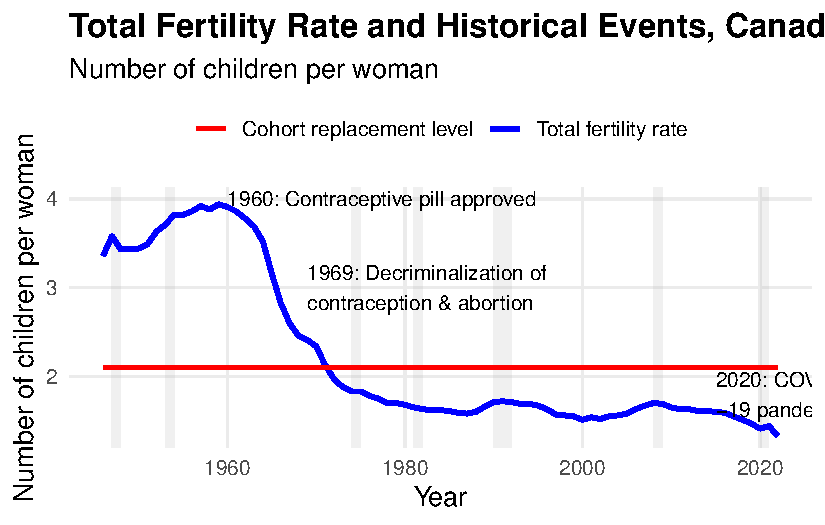
\includegraphics{paper_files/figure-pdf/unnamed-chunk-4-1.pdf}

\begin{Shaded}
\begin{Highlighting}[]
\FunctionTok{library}\NormalTok{(tidyverse)}
\end{Highlighting}
\end{Shaded}

\begin{verbatim}
Warning: package 'tibble' was built under R version 4.4.3
\end{verbatim}

\begin{verbatim}
Warning: package 'purrr' was built under R version 4.4.3
\end{verbatim}

\begin{verbatim}
Warning: package 'forcats' was built under R version 4.4.3
\end{verbatim}

\begin{verbatim}
Warning: package 'lubridate' was built under R version 4.4.3
\end{verbatim}

\begin{verbatim}
-- Attaching core tidyverse packages ------------------------ tidyverse 2.0.0 --
v forcats   1.0.1     v tibble    3.3.0
v lubridate 1.9.4     v tidyr     1.3.1
v purrr     1.1.0     
-- Conflicts ------------------------------------------ tidyverse_conflicts() --
x dplyr::filter() masks stats::filter()
x dplyr::lag()    masks stats::lag()
i Use the conflicted package (<http://conflicted.r-lib.org/>) to force all conflicts to become errors
\end{verbatim}

\begin{Shaded}
\begin{Highlighting}[]
\CommentTok{\# {-}{-}{-} Step 1: Read data {-}{-}{-}}
\NormalTok{death }\OtherTok{\textless{}{-}} \FunctionTok{read\_csv}\NormalTok{(}\StringTok{"Canada\_Death.csv"}\NormalTok{)}
\end{Highlighting}
\end{Shaded}

\begin{verbatim}
New names:
Rows: 1357 Columns: 7
-- Column specification
-------------------------------------------------------- Delimiter: "," chr
(3): country, sex, cause dbl (3): year, age_group, death lgl (1): ...7
i Use `spec()` to retrieve the full column specification for this data. i
Specify the column types or set `show_col_types = FALSE` to quiet this message.
* `` -> `...7`
\end{verbatim}

\begin{Shaded}
\begin{Highlighting}[]
\CommentTok{\# {-}{-}{-} Step 2: Filter for 2000–2022, age 0, Canada, and selected causes {-}{-}{-}}
\NormalTok{death\_dot }\OtherTok{\textless{}{-}}\NormalTok{ death }\SpecialCharTok{\%\textgreater{}\%}
  \FunctionTok{filter}\NormalTok{(country }\SpecialCharTok{==} \StringTok{"Canada"}\NormalTok{,}
\NormalTok{         year }\SpecialCharTok{\textgreater{}=} \DecValTok{2000}\NormalTok{, year }\SpecialCharTok{\textless{}=} \DecValTok{2022}\NormalTok{,}
\NormalTok{         age\_group }\SpecialCharTok{==} \StringTok{"0"}\NormalTok{,}
\NormalTok{         cause }\SpecialCharTok{\%in\%} \FunctionTok{c}\NormalTok{(}\StringTok{"I050"}\NormalTok{, }\StringTok{"I051"}\NormalTok{, }\StringTok{"I058"}\NormalTok{)) }\SpecialCharTok{\%\textgreater{}\%}
  \FunctionTok{group\_by}\NormalTok{(year, cause) }\SpecialCharTok{\%\textgreater{}\%}
  \FunctionTok{summarise}\NormalTok{(}\AttributeTok{total\_deaths =} \FunctionTok{sum}\NormalTok{(death, }\AttributeTok{na.rm =} \ConstantTok{TRUE}\NormalTok{), }\AttributeTok{.groups =} \StringTok{"drop"}\NormalTok{)}

\CommentTok{\# {-}{-}{-} Step 3: Plot colored dots + separate gray dashed lines per cause {-}{-}{-}}
\FunctionTok{ggplot}\NormalTok{(death\_dot, }\FunctionTok{aes}\NormalTok{(}\AttributeTok{x =}\NormalTok{ year, }\AttributeTok{y =}\NormalTok{ total\_deaths, }\AttributeTok{color =}\NormalTok{ cause)) }\SpecialCharTok{+}
  
  \CommentTok{\# {-}{-}{-} Colored dots for each cause {-}{-}{-}}
  \FunctionTok{geom\_point}\NormalTok{(}\AttributeTok{size =} \DecValTok{3}\NormalTok{, }\AttributeTok{alpha =} \FloatTok{0.6}\NormalTok{) }\SpecialCharTok{+}
  
  \CommentTok{\# {-}{-}{-} Individual gray dashed fitted lines for each cause {-}{-}{-}}
  \FunctionTok{geom\_smooth}\NormalTok{(}
    \FunctionTok{aes}\NormalTok{(}\AttributeTok{group =}\NormalTok{ cause),   }\CommentTok{\# separate line per cause}
    \AttributeTok{method =} \StringTok{"lm"}\NormalTok{, }\AttributeTok{se =} \ConstantTok{FALSE}\NormalTok{, }\AttributeTok{color =} \StringTok{"gray60"}\NormalTok{,}
    \AttributeTok{linewidth =} \DecValTok{1}\NormalTok{, }\AttributeTok{linetype =} \StringTok{"dashed"}
\NormalTok{  ) }\SpecialCharTok{+}
  
  \CommentTok{\# {-}{-}{-} Custom colors for dots {-}{-}{-}}
  \FunctionTok{scale\_color\_manual}\NormalTok{(}
    \AttributeTok{values =} \FunctionTok{c}\NormalTok{(}
      \StringTok{"I050"} \OtherTok{=} \StringTok{"\#E57373"}\NormalTok{,   }\CommentTok{\# red}
      \StringTok{"I051"} \OtherTok{=} \StringTok{"\#66BB6A"}\NormalTok{,   }\CommentTok{\# green}
      \StringTok{"I058"} \OtherTok{=} \StringTok{"\#64B5F6"}    \CommentTok{\# blue}
\NormalTok{    ),}
    \AttributeTok{labels =} \FunctionTok{c}\NormalTok{(}
      \StringTok{"I050 – Perinatal conditions"}\NormalTok{,}
      \StringTok{"I051 – Congenital malformations"}\NormalTok{,}
      \StringTok{"I058 – Ill{-}defined causes"}
\NormalTok{    ),}
    \AttributeTok{name =} \StringTok{"Cause"}
\NormalTok{  ) }\SpecialCharTok{+}
  
  \CommentTok{\# {-}{-}{-} Labels and titles {-}{-}{-}}
  \FunctionTok{labs}\NormalTok{(}
    \AttributeTok{title =} \StringTok{"Infant Mortality in Canada (2000–2022)"}\NormalTok{,}
    \AttributeTok{subtitle =} \StringTok{"Age group: 0 years; Three selected causes with individual gray trend lines"}\NormalTok{,}
    \AttributeTok{x =} \StringTok{"Year"}\NormalTok{,}
    \AttributeTok{y =} \StringTok{"Total Deaths"}
\NormalTok{  ) }\SpecialCharTok{+}
  
  \CommentTok{\# {-}{-}{-} Style {-}{-}{-}}
  \FunctionTok{theme\_minimal}\NormalTok{(}\AttributeTok{base\_size =} \DecValTok{14}\NormalTok{) }\SpecialCharTok{+}
  \FunctionTok{theme}\NormalTok{(}
    \AttributeTok{legend.position =} \StringTok{"right"}\NormalTok{,}
    \AttributeTok{legend.title =} \FunctionTok{element\_text}\NormalTok{(}\AttributeTok{size =} \DecValTok{10}\NormalTok{, }\AttributeTok{face =} \StringTok{"bold"}\NormalTok{),}
    \AttributeTok{legend.text =} \FunctionTok{element\_text}\NormalTok{(}\AttributeTok{size =} \DecValTok{9}\NormalTok{),}
    \AttributeTok{plot.title =} \FunctionTok{element\_text}\NormalTok{(}\AttributeTok{face =} \StringTok{"bold"}\NormalTok{, }\AttributeTok{size =} \DecValTok{16}\NormalTok{, }\AttributeTok{color =} \StringTok{"\#222"}\NormalTok{),}
    \AttributeTok{plot.subtitle =} \FunctionTok{element\_text}\NormalTok{(}\AttributeTok{size =} \DecValTok{12}\NormalTok{, }\AttributeTok{color =} \StringTok{"\#555"}\NormalTok{),}
    \AttributeTok{panel.grid.minor =} \FunctionTok{element\_blank}\NormalTok{(),}
    \AttributeTok{panel.grid.major =} \FunctionTok{element\_line}\NormalTok{(}\AttributeTok{color =} \StringTok{"gray90"}\NormalTok{, }\AttributeTok{linewidth =} \FloatTok{0.3}\NormalTok{)}
\NormalTok{  )}
\end{Highlighting}
\end{Shaded}

\begin{verbatim}
`geom_smooth()` using formula = 'y ~ x'
\end{verbatim}

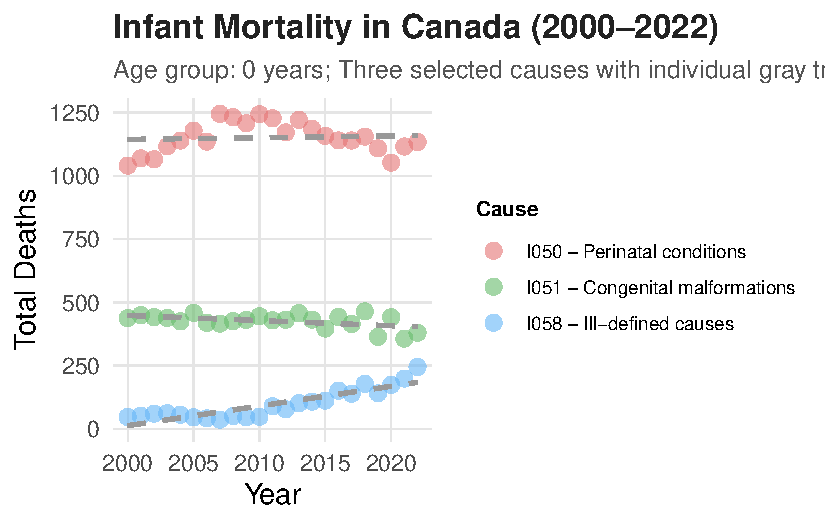
\includegraphics{paper_files/figure-pdf/unnamed-chunk-5-1.pdf}




\end{document}
